% ┌────────────────────────────────────────────────────────────────────────────┐
% │ ANGIO PAPER                                                                │
% │   Endoscopic hemostasis makes the difference: Angiographic treatment in    │
% │   patients with lower gastrointestinal bleeding                            │
% └────────────────────────────────────────────────────────────────────────────┘

\chapter{Angiography for Gastrointestinal Bleeding}
This study




\vspace{2,5cm}

\begin{figure}[h!]
\centering
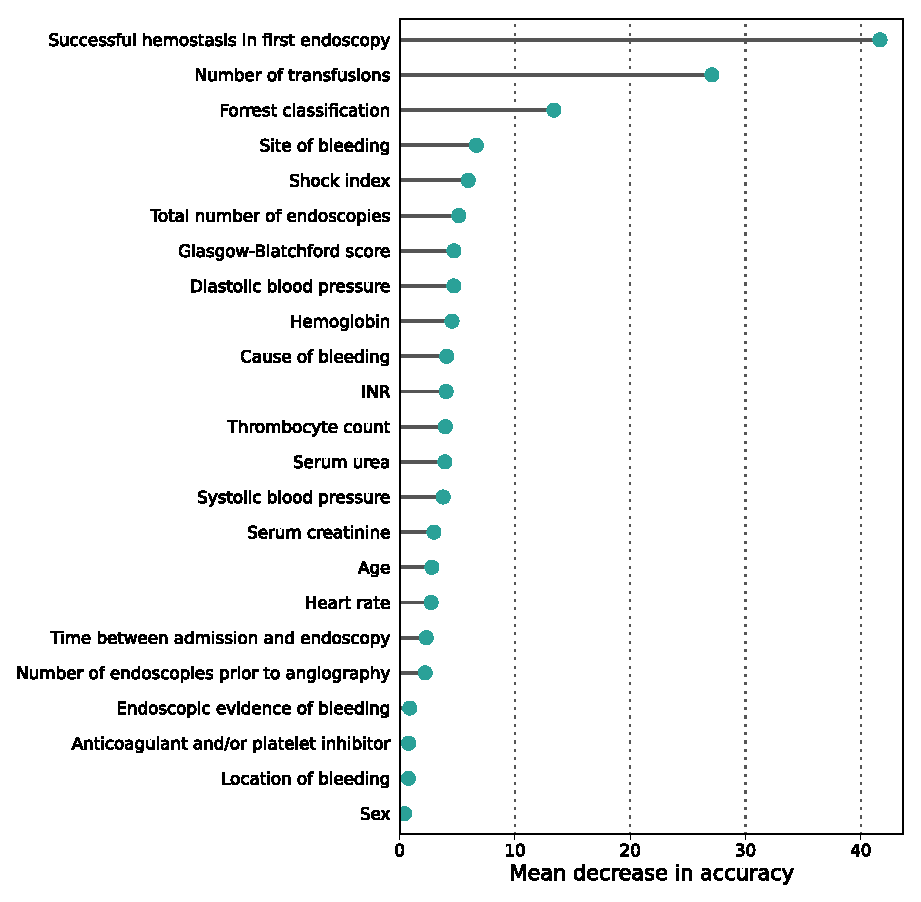
\includegraphics[width=\textwidth]{04_GraphicFiles/angiography.eps}
\caption{Modification of figure 1 from \citet{Werner2021}.}
\label{fig:angio}
\end{figure}

% \section{Project Introduction}

% \section{Failed Explorations}

% \section{Decision Trees for Diagnostic Support}

\vfill
\noindent My contribution to this publication was the complete bioinformatic
and statistical analysis.\nopagebreak
\medskip
\begin{tcolorbox}[
  boxrule=0pt, leftrule=1pt, colframe=s-blue, colback=white, sharp corners=all]%
  \raggedright
  Werner, DJ., Baar, T., Kiesslich, R., Wenzel, N., Abusalim, N., Tresch, A.,
  Rey, JW. (2021).
  
  \smallskip
  \href{https://www.wjgnet.com/1948-5190/full/v13/i7/221.htm}
    {Endoscopic hemostasis makes the difference: Angiographic treatment in
    patients with lower gastrointestinal bleeding}

  \smallskip
  \textit{World J Gastrointest Endosc, 13(7): 221-232}
\end{tcolorbox}

% ┌────────────────────────────────────────────────────────────────────────────┐
% │ PDF                                                                        │
% └────────────────────────────────────────────────────────────────────────────┘

% \includepdf[pages={4-15}, addtotoc={4, section, 1,
%   Endoscopic hemostasis makes the difference: Angiographic treatment in
%   patients with lower gastrointestinal bleeding,
%   Endoscopic hemostasis makes the difference: Angiographic treatment in
%   patients with lower gastrointestinal bleeding}]
%   {"99_Publications/Werner2021.pdf"}